\subsubsection{TimeFrame::v1::Header}
総長は24 byteである。識別子は\texttt{0x004d5246454d4954}である。
\begin{longtable}{r r l p{0.40\linewidth}}
\caption{TimeFrame::v1::Headerのフィールド配置。}\label{tab:format-tf}\\
\hline オフセット & byte数 & フィールド & 意味 \\ \hline\endfirsthead
\hline オフセット & byte数 & フィールド & 意味 \\ \hline\endhead
0 & 8 & \texttt{magic} &  \\
8 & 4 & \texttt{length} & 自分のヘッダを含むフレーム長 [byte] \\
12 & 2 & \texttt{hLength} & ヘッダ長 [byte] \\
14 & 2 & \texttt{type} &  \\
16 & 4 & \texttt{timeFrameId} & 集約するSTFと対応するID \\
20 & 4 & \texttt{numSource} & TFに含めるソース数 \\
\hline\end{longtable}
\begin{figure}[htbp]\centering\makebox[\linewidth][c]{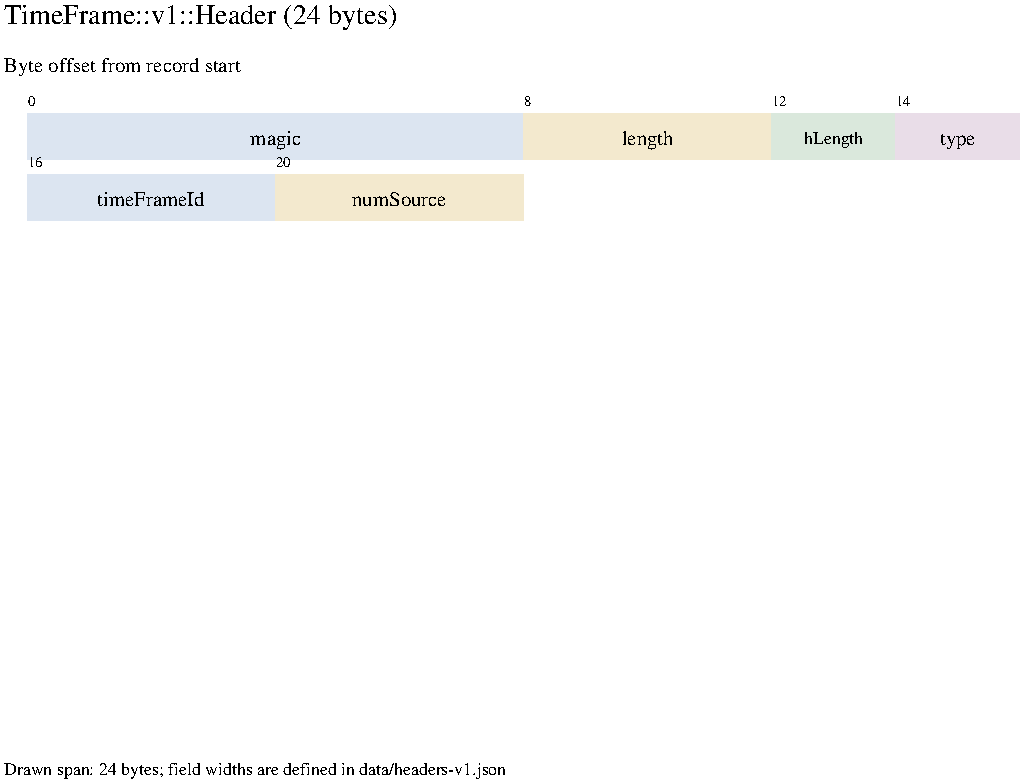
\includegraphics[pagebox=cropbox,width=0.95\linewidth,height=0.55\textheight,keepaspectratio]{../figure/10-3-nestdaq-dataformat/pdf/tf.pdf}}\caption{TimeFrame::v1::Headerのバイト配置。}\label{fig:format-tf}\end{figure}
\subsubsection{SubTimeFrame::v1::Header}
総長は48 byteである。識別子は\texttt{0x00454d4954425553}である。
\begin{longtable}{r r l p{0.40\linewidth}}
\caption{SubTimeFrame::v1::Headerのフィールド配置。}\label{tab:format-stf}\\
\hline オフセット & byte数 & フィールド & 意味 \\ \hline\endfirsthead
\hline オフセット & byte数 & フィールド & 意味 \\ \hline\endhead
0 & 8 & \texttt{magic} &  \\
8 & 4 & \texttt{length} & 自分のヘッダを含むフレーム長 [byte] \\
12 & 2 & \texttt{hLength} & ヘッダ長 [byte] \\
14 & 2 & \texttt{type} &  \\
16 & 4 & \texttt{timeFrameId} & STFBuilderの設定によりHBD由来IDまたは連番 \\
20 & 4 & \texttt{femType} & FEM種別・データ世代の識別 \\
24 & 4 & \texttt{femId} & FEM識別子 \\
28 & 4 & \texttt{numMessages} & STFBuilderではSTFヘッダを除くpayloadメッセージ数 \\
32 & 8 & \texttt{timeSec} & STFBuilderではgettimeofday().tv\_sec \\
40 & 8 & \texttt{timeUSec} & STFBuilderではgettimeofday().tv\_usec：秒内のµs \\
\hline\end{longtable}
\begin{figure}[htbp]\centering\makebox[\linewidth][c]{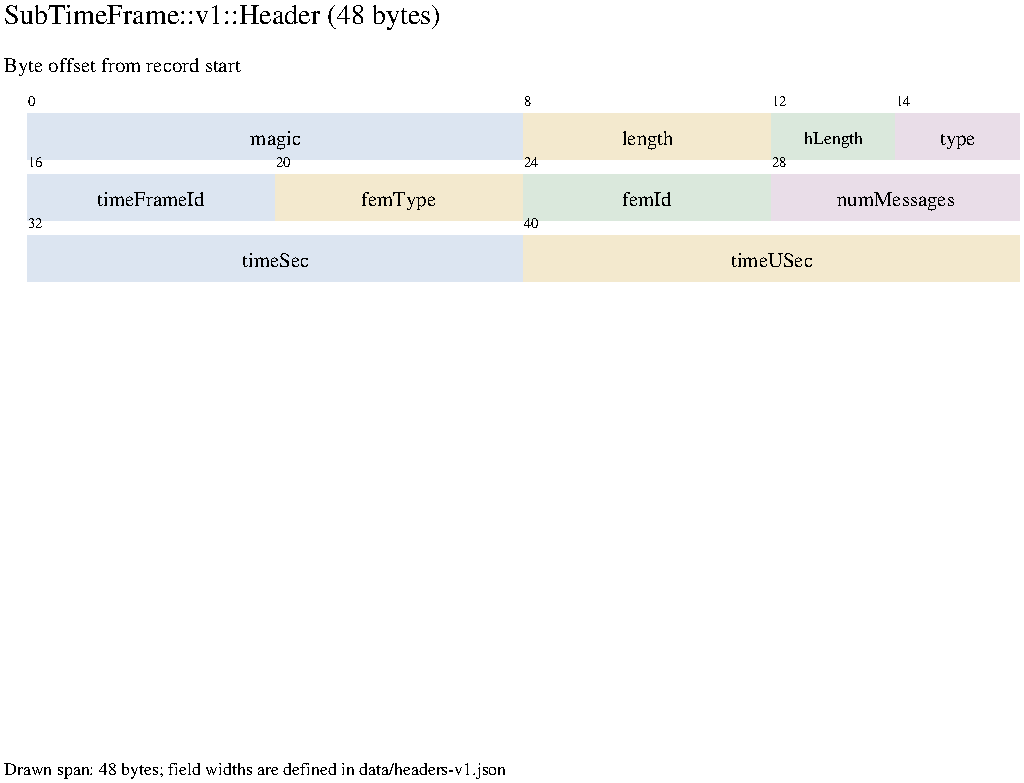
\includegraphics[pagebox=cropbox,width=0.95\linewidth,height=0.55\textheight,keepaspectratio]{../figure/10-3-nestdaq-dataformat/pdf/stf.pdf}}\caption{SubTimeFrame::v1::Headerのバイト配置。}\label{fig:format-stf}\end{figure}
\subsubsection{HeartbeatFrame::Header}
総長は16 byteである。識別子は\texttt{0x0054414542545248}である。
\begin{longtable}{r r l p{0.40\linewidth}}
\caption{HeartbeatFrame::Headerのフィールド配置。}\label{tab:format-hbf}\\
\hline オフセット & byte数 & フィールド & 意味 \\ \hline\endfirsthead
\hline オフセット & byte数 & フィールド & 意味 \\ \hline\endhead
0 & 8 & \texttt{magic} &  \\
8 & 4 & \texttt{length} & 自分のヘッダを含むフレーム長 [byte] \\
12 & 2 & \texttt{hLength} & ヘッダ長 [byte] \\
14 & 2 & \texttt{type} &  \\
\hline\end{longtable}
\begin{figure}[htbp]\centering\makebox[\linewidth][c]{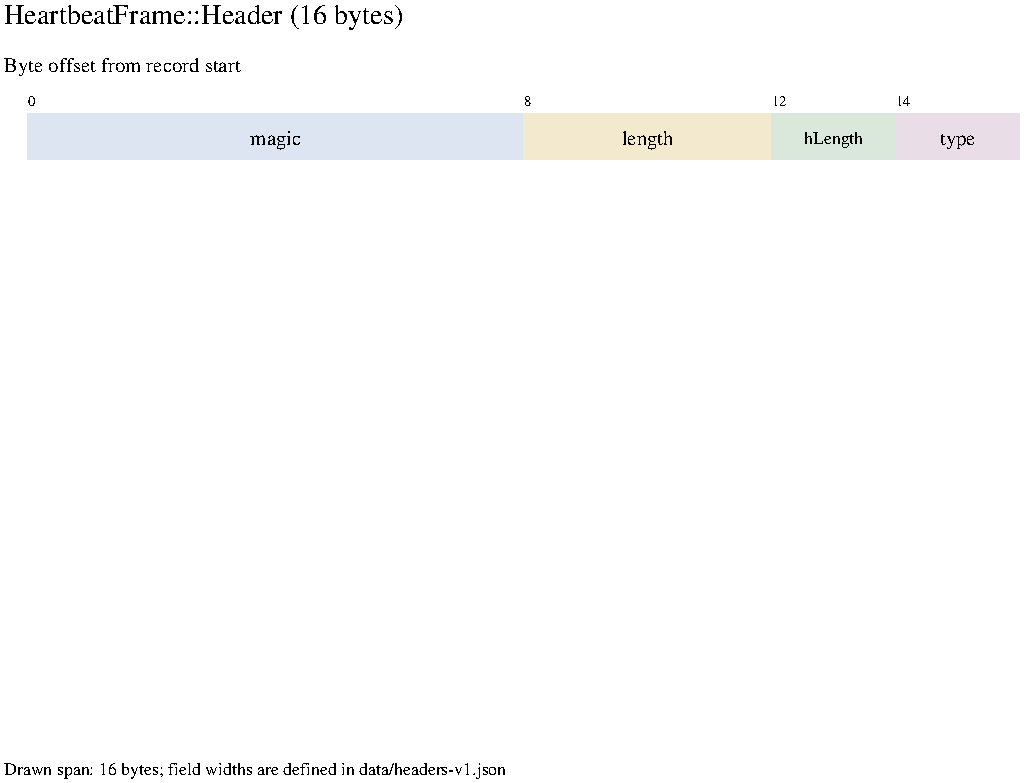
\includegraphics[pagebox=cropbox,width=0.95\linewidth,height=0.55\textheight,keepaspectratio]{../figure/10-3-nestdaq-dataformat/pdf/hbf.pdf}}\caption{HeartbeatFrame::Headerのバイト配置。}\label{fig:format-hbf}\end{figure}
\subsubsection{Filter::v1::Header}
総長は56 byteである。識別子は\texttt{0x0049474f4c544c46}である。
\begin{longtable}{r r l p{0.40\linewidth}}
\caption{Filter::v1::Headerのフィールド配置。}\label{tab:format-filter}\\
\hline オフセット & byte数 & フィールド & 意味 \\ \hline\endfirsthead
\hline オフセット & byte数 & フィールド & 意味 \\ \hline\endhead
0 & 8 & \texttt{magic} &  \\
8 & 4 & \texttt{length} & 自分のヘッダを含むフレーム長 [byte] \\
12 & 2 & \texttt{hLength} & ヘッダ長 [byte] \\
14 & 2 & \texttt{type} &  \\
16 & 4 & \texttt{timeFrameId} &  \\
20 & 4 & \texttt{numTrigs} & LogicFilterでは全HBFのtrigger数の合計 \\
24 & 4 & \texttt{workerId} &  \\
28 & 4 & \texttt{numMessages} & LogicFilterでは1 + Trigger Timeブロック数 \\
32 & 4 & \texttt{elapseTime} & LogicFilterの処理経過時間 [µs] \\
36 & 4 & \texttt{reserve} & 初期値0xff00ff00 \\
40 & 8 & \texttt{timeSec} & LogicFilterではepochからの秒 \\
48 & 8 & \texttt{timeUSec} & LogicFilterではepochからの総µs。STFのtimeUSecとは意味が異なる \\
\hline\end{longtable}
\begin{figure}[htbp]\centering\makebox[\linewidth][c]{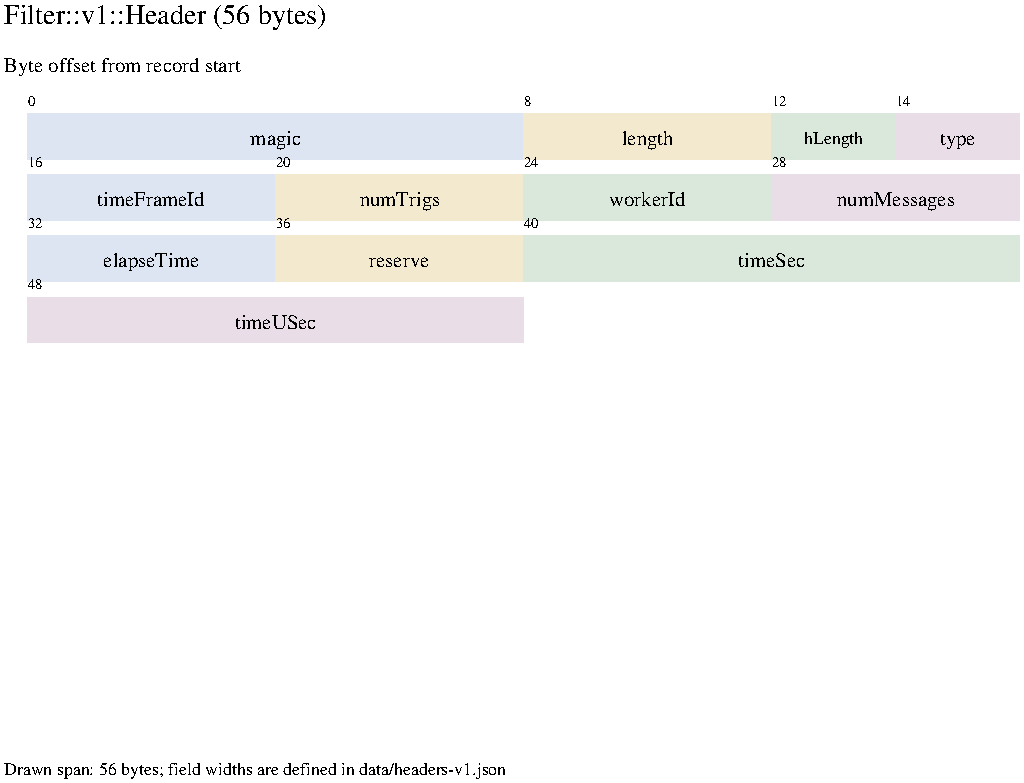
\includegraphics[pagebox=cropbox,width=0.95\linewidth,height=0.55\textheight,keepaspectratio]{../figure/10-3-nestdaq-dataformat/pdf/filter.pdf}}\caption{Filter::v1::Headerのバイト配置。}\label{fig:format-filter}\end{figure}
\subsubsection{Filter::v1::TrgTimeHeader}
総長は16 byteである。識別子は\texttt{0x00454d4954475254}である。
\begin{longtable}{r r l p{0.40\linewidth}}
\caption{Filter::v1::TrgTimeHeaderのフィールド配置。}\label{tab:format-trigger}\\
\hline オフセット & byte数 & フィールド & 意味 \\ \hline\endfirsthead
\hline オフセット & byte数 & フィールド & 意味 \\ \hline\endhead
0 & 8 & \texttt{magic} &  \\
8 & 4 & \texttt{length} & 自分のヘッダを含むフレーム長 [byte] \\
12 & 2 & \texttt{hLength} & ヘッダ長 [byte] \\
14 & 2 & \texttt{type} &  \\
\hline\end{longtable}
\begin{figure}[htbp]\centering\makebox[\linewidth][c]{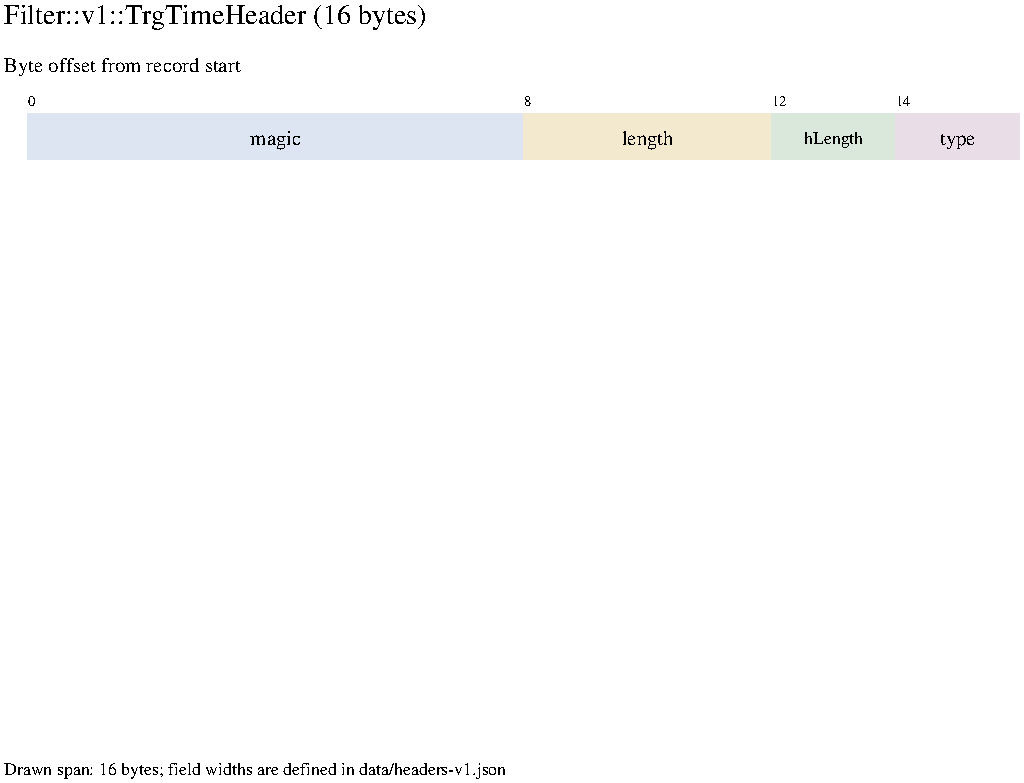
\includegraphics[pagebox=cropbox,width=0.95\linewidth,height=0.55\textheight,keepaspectratio]{../figure/10-3-nestdaq-dataformat/pdf/trigger.pdf}}\caption{Filter::v1::TrgTimeHeaderのバイト配置。}\label{fig:format-trigger}\end{figure}
\subsubsection{FileSinkHeader::v1::Header}
総長は304 byteである。識別子は\texttt{0x004b4e53454c4946}である。
\begin{longtable}{r r l p{0.40\linewidth}}
\caption{FileSinkHeader::v1::Headerのフィールド配置。}\label{tab:format-file-header}\\
\hline オフセット & byte数 & フィールド & 意味 \\ \hline\endfirsthead
\hline オフセット & byte数 & フィールド & 意味 \\ \hline\endhead
0 & 8 & \texttt{magic} &  \\
8 & 4 & \texttt{length} & 自分のヘッダを含むフレーム長 [byte] \\
12 & 2 & \texttt{hLength} & ヘッダ長 [byte] \\
14 & 2 & \texttt{type} &  \\
16 & 8 & \texttt{fairMQDeviceType} & FileSinkのHeaderで99に設定 \\
24 & 8 & \texttt{runNumber} &  \\
32 & 8 & \texttt{startUnixtime} & run開始時刻。ここではtime\_t=8を仮定 \\
40 & 8 & \texttt{stopUnixtime} & Headerでは0、Trailerでは終了時刻 \\
48 & 256 & \texttt{comments} & runコメント \\
\hline\end{longtable}
\begin{figure}[htbp]\centering\makebox[\linewidth][c]{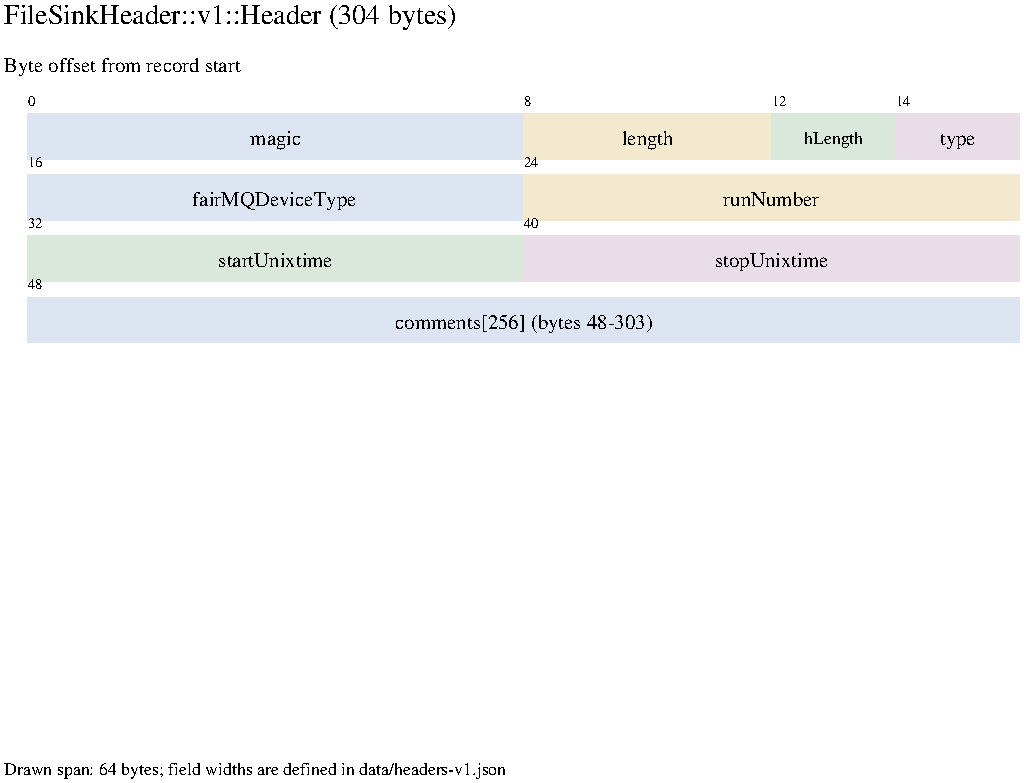
\includegraphics[pagebox=cropbox,width=0.95\linewidth,height=0.55\textheight,keepaspectratio]{../figure/10-3-nestdaq-dataformat/pdf/file-header.pdf}}\caption{FileSinkHeader::v1::Headerのバイト配置。commentsは256 byteを1段に縮約して示す。}\label{fig:format-file-header}\end{figure}
\subsubsection{FileSinkTrailer::v1::Trailer}
総長は304 byteである。識別子は\texttt{0x004c5254454c4946}である。
\begin{longtable}{r r l p{0.40\linewidth}}
\caption{FileSinkTrailer::v1::Trailerのフィールド配置。}\label{tab:format-file-trailer}\\
\hline オフセット & byte数 & フィールド & 意味 \\ \hline\endfirsthead
\hline オフセット & byte数 & フィールド & 意味 \\ \hline\endhead
0 & 8 & \texttt{magic} &  \\
8 & 4 & \texttt{length} & 自分のヘッダを含むフレーム長 [byte] \\
12 & 2 & \texttt{hLength} & ヘッダ長 [byte] \\
14 & 2 & \texttt{type} &  \\
16 & 8 & \texttt{fairMQDeviceType} & FileSinkのHeaderで99に設定 \\
24 & 8 & \texttt{runNumber} &  \\
32 & 8 & \texttt{startUnixtime} & run開始時刻。ここではtime\_t=8を仮定 \\
40 & 8 & \texttt{stopUnixtime} & Headerでは0、Trailerでは終了時刻 \\
48 & 256 & \texttt{comments} & runコメント \\
\hline\end{longtable}
\begin{figure}[htbp]\centering\makebox[\linewidth][c]{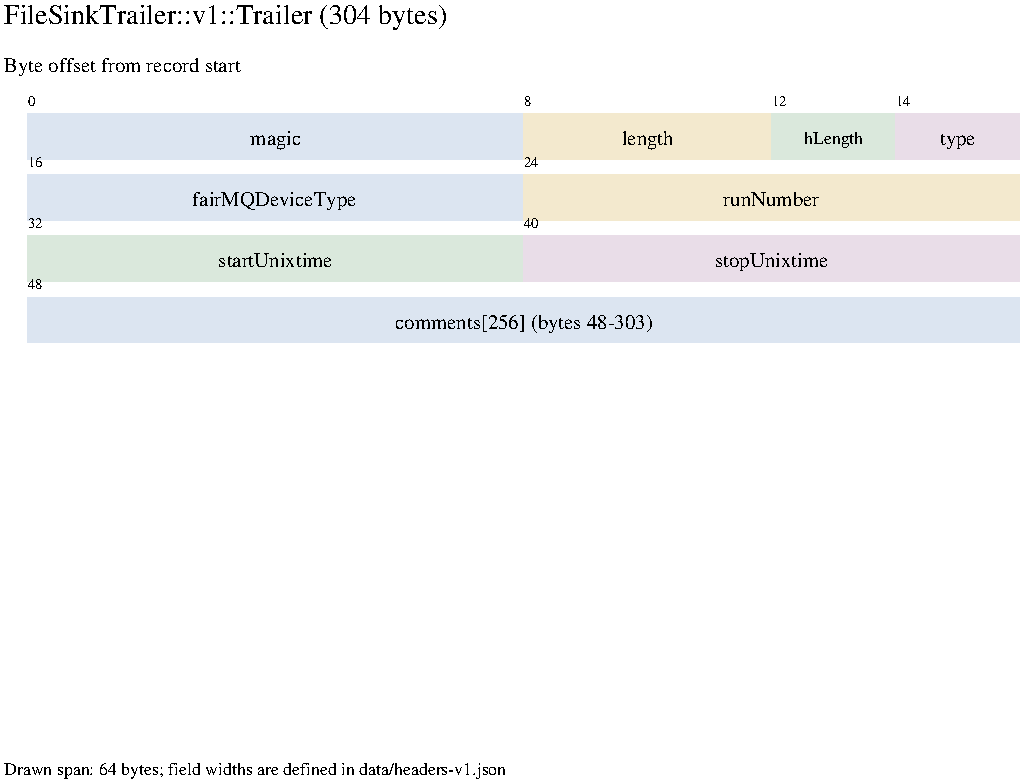
\includegraphics[pagebox=cropbox,width=0.95\linewidth,height=0.55\textheight,keepaspectratio]{../figure/10-3-nestdaq-dataformat/pdf/file-trailer.pdf}}\caption{FileSinkTrailer::v1::Trailerのバイト配置。commentsは256 byteを1段に縮約して示す。}\label{fig:format-file-trailer}\end{figure}
\subsubsection{Filter::v1::TrgTime}
総長は8 byteである。
\begin{longtable}{r r l p{0.40\linewidth}}
\caption{Filter::v1::TrgTimeのフィールド配置。}\label{tab:format-trgtime}\\
\hline オフセット & byte数 & フィールド & 意味 \\ \hline\endfirsthead
\hline オフセット & byte数 & フィールド & 意味 \\ \hline\endhead
0 & 4 & \texttt{time} & trigger時刻。Slicerはtdc4nと比較する \\
4 & 4 & \texttt{type} & LogicFilterは0xaa000000を出力。little-endian末尾byteは0xaa \\
\hline\end{longtable}
\begin{figure}[htbp]\centering\makebox[\linewidth][c]{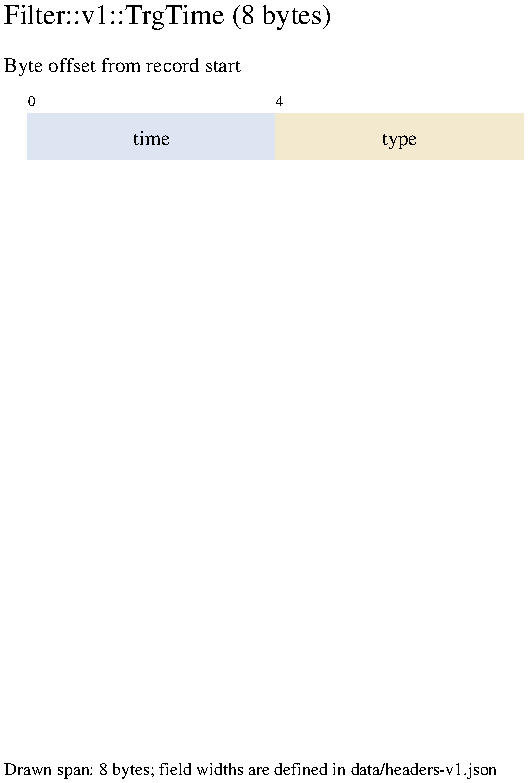
\includegraphics[pagebox=cropbox,width=0.95\linewidth,height=0.55\textheight,keepaspectratio]{../figure/10-3-nestdaq-dataformat/pdf/trgtime.pdf}}\caption{Filter::v1::TrgTimeのバイト配置。}\label{fig:format-trgtime}\end{figure}
